\section{レポート課題2}
\subsection{課題1}
ジスティク写像で$r = 1.50, r = 2.60, r = 3.20, r = 3.50, r = 3.86, r = 3.90$として、初期値$x_0$を$0$から$1$まで$0.001$きざみで変化させたときの、$x_{200}$の値がどうなっているかグラフ化せよ。また、$x_n$が$150 < n < 200$の場合もグラフ化せよ。出力形式は授業資料を参照すること。\par
画像:
\begin{figure}[h]
  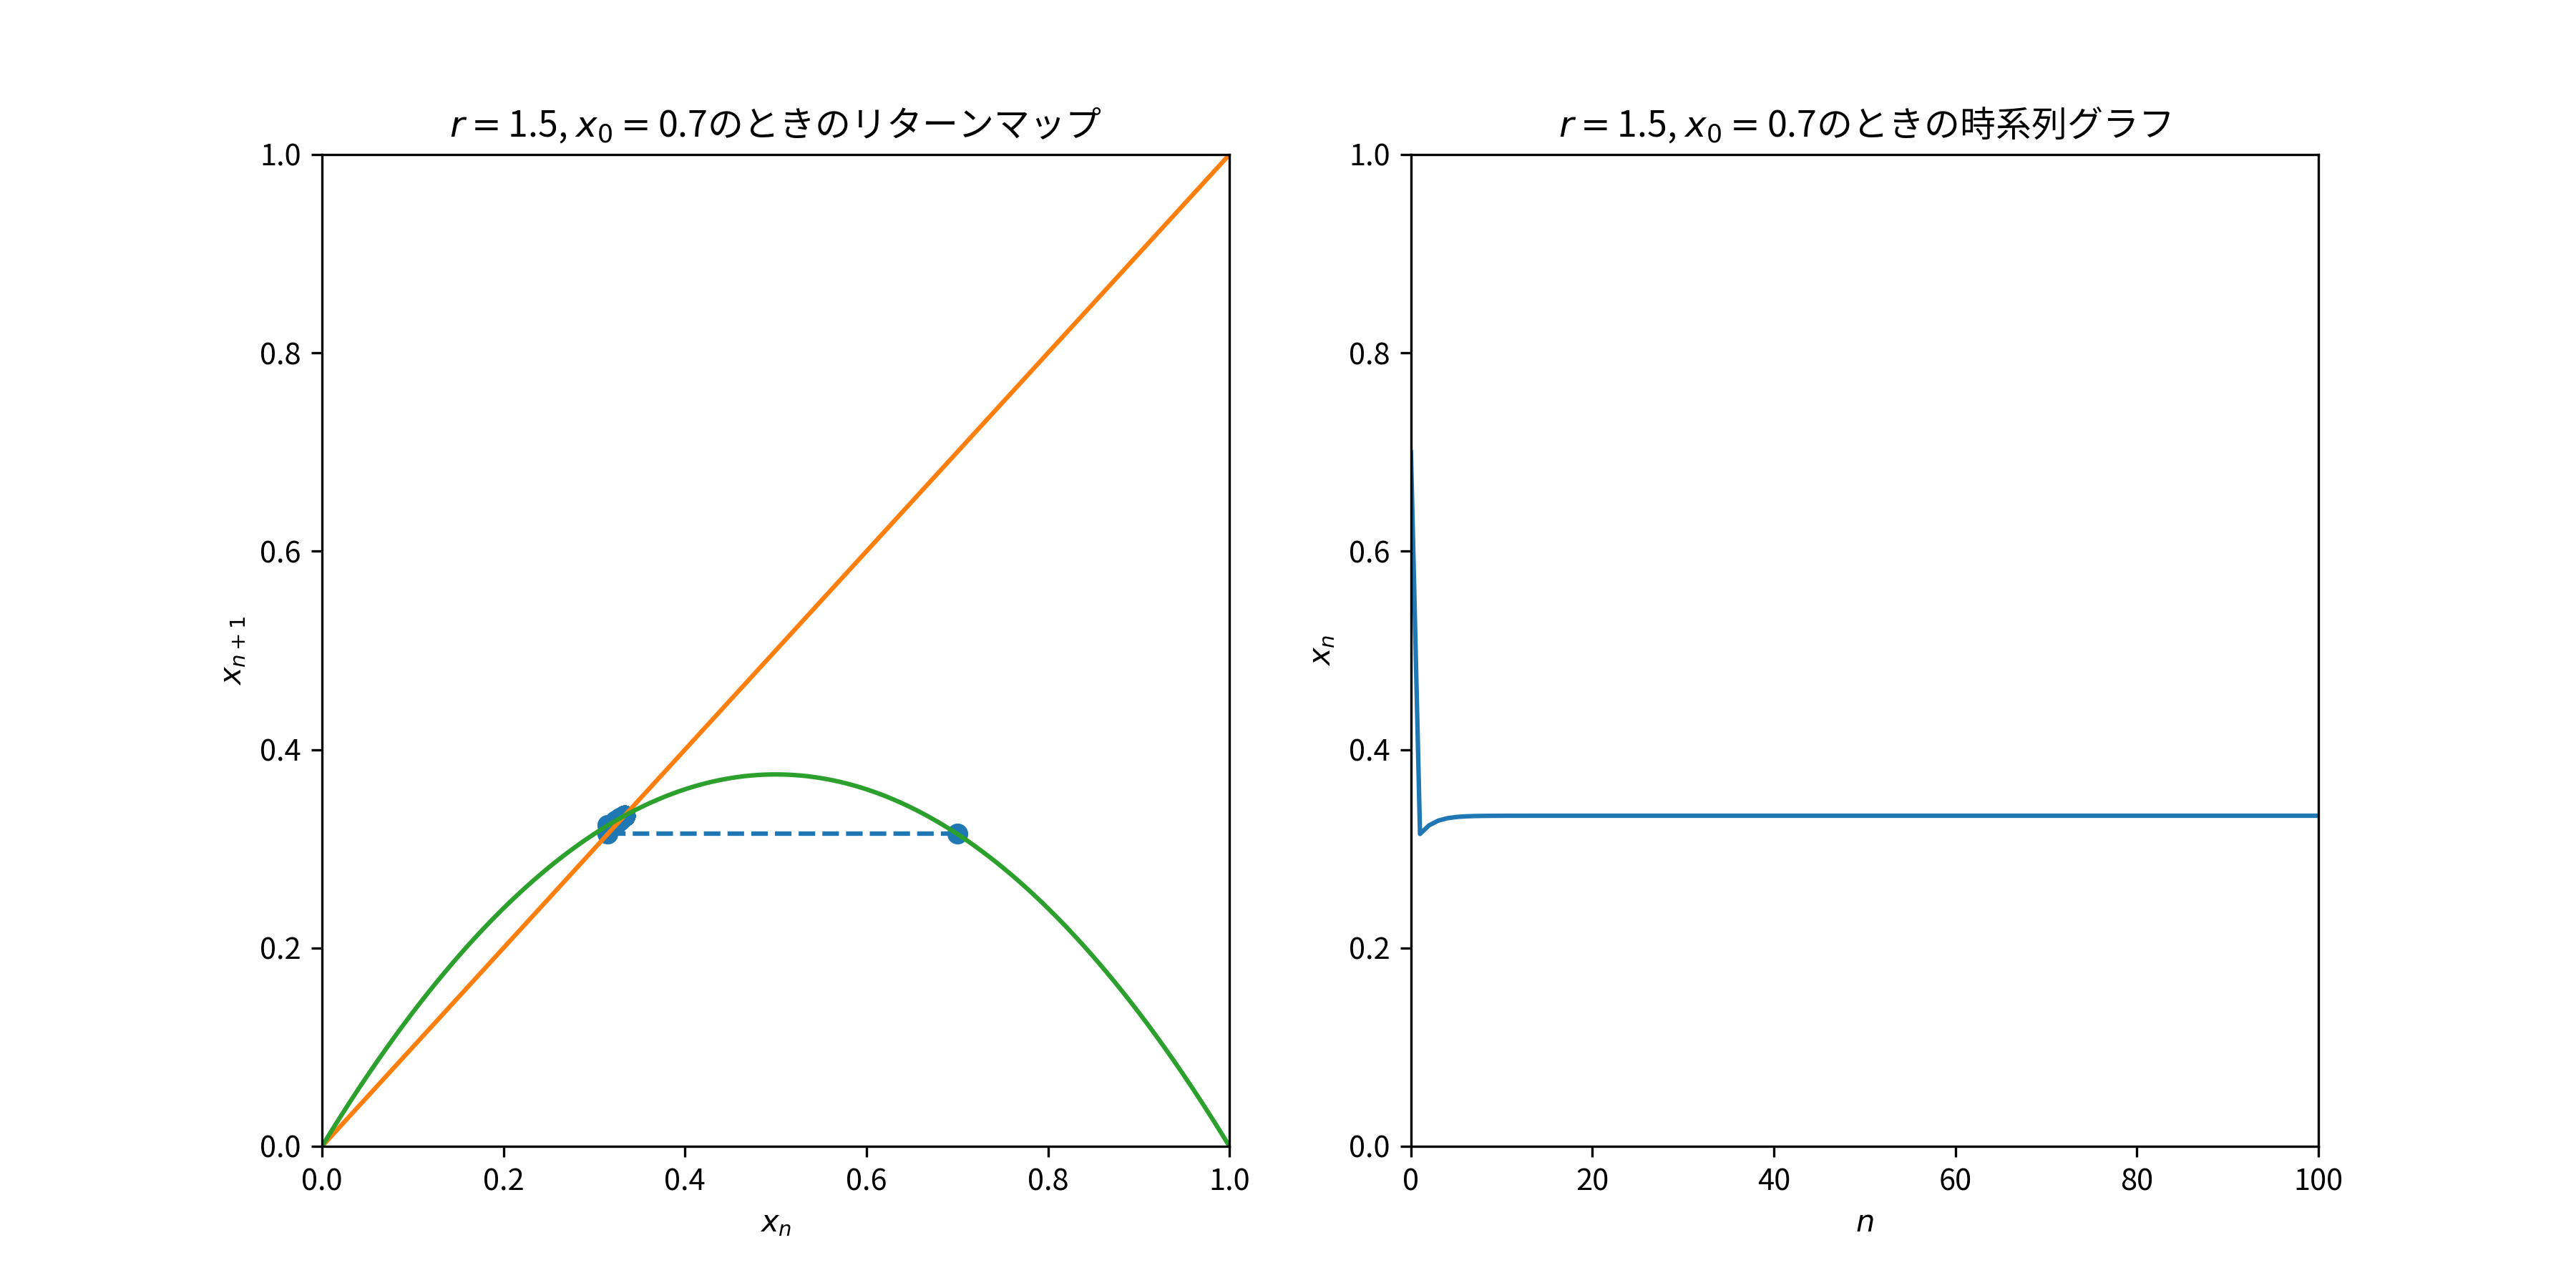
\includegraphics[width=15cm]{images/ctest2_1.png}
\end{figure}

解説:\par
この図は左にリターンマップ、右に時系列グラフをプロットした図をレポートの

\subsection{課題2}
課題1 で得られた結果から初期値鋭敏性を説明せよ。